\section{Results}
\label{sec:results}

We report results organized by our four questions. We present expected qualitative patterns consistent with the protocol of Section~\ref{sec:experimental-setup}; full quantitative tables will be populated upon completion of the runs, and the structure here reflects the analyses we will report. Throughout, ``M1'' denotes ResponseVec and ``M2'' denotes RespondentVec; B1--B7 denote the baselines of Section~\ref{sec:baselines}, and ``M3'' denotes the mixed allocation policy of Section~\ref{sec:tradeoff}.

\subsection{Q1: Unseen-Item Accuracy and Calibration}
\label{sec:results-q1}

Table~\ref{tab:within} reports accuracy, NLL, RPS, Brier score, and ECE on the unseen-item regime (R1), where every candidate target item is held out in exactly one of the six outer folds. We anticipate that direct generation (B1, even with its strongest neural calibrator) will lag representation-based methods on calibration, because a single option-token readout provides no faithful uncertainty over the option simplex; that the classical psychometric baselines (B2 majority/MIRT, B3 item-conditional CF) will be competitive on items where collaborative structure is strong but will refuse to predict unseen items (MIRT) or fall back to the prior, exposing the limit of non-semantic models; and that QLoRA (B4) will achieve the highest raw accuracy at the highest compute cost. We expect M1 (ResponseVec) to match or exceed B4 on accuracy while being far cheaper, and to substantially improve ECE relative to all direct-generation baselines owing to the calibratable decoder. M2 (RespondentVec) should trail M1 on accuracy but match its calibration advantage.

\begin{table}[tb]
\centering
\small
\caption{Unseen-item (R1) results. Accuracy (Acc), NLL ($\downarrow$), RPS ($\downarrow$), Brier (Br, $\downarrow$), ECE ($\downarrow$), and GPU-hours per 1000 respondents. Mean$\pm$std over 3 decoder seeds $\times$ 3 option seeds. Best in \textbf{bold}; second best \underline{underlined}.}
\label{tab:within}
\begin{tabular}{lcccccr}
\toprule
Method & Acc & NLL$\downarrow$ & RPS$\downarrow$ & Br$\downarrow$ & ECE$\downarrow$ & GPU-h$\downarrow$ \\
\midrule
B1 Direct gen.\ (best calib.) & --- & --- & --- & --- & --- & --- \\
B2 Majority + MIRT            & --- & --- & --- & --- & --- & --- \\
B3 Item-conditional CF        & --- & --- & --- & --- & --- & --- \\
B4 QLoRA                      & --- & --- & --- & --- & --- & --- \\
B5 Generic text vector        & --- & --- & --- & --- & --- & --- \\
B6 Raw hidden states          & --- & --- & --- & --- & --- & --- \\
B7 LLM2Vec (no Gen)           & --- & --- & --- & --- & --- & --- \\
\midrule
M2 RespondentVec              & --- & --- & --- & --- & --- & --- \\
M1 ResponseVec                & --- & --- & --- & --- & --- & --- \\
\bottomrule
\end{tabular}
\end{table}

\subsection{Q2: Three-Way Transfer}
\label{sec:results-q2}

Table~\ref{tab:transfer} reports accuracy under the three transfer regimes---R1 unseen-item (reference), R2 cross-domain (leave-one-domain-out), and R3 OOD-demographic-intersection---together with the transfer ratio $\rho$ relative to R1. Figure~\ref{fig:transfer} visualizes the degradation trajectories. We anticipate three patterns matching the predictions of Section~\ref{sec:tradeoff}. First, all methods degrade from R1 to R2, but direct-generation methods (B1) degrade most because their option-token readouts are overfit to the training domain's option phrasings; representation-based methods degrade less because the option-aware decoder generalizes across option sets. Second, the cross-domain regime (R2) penalizes methods that couple the encoder to a specific content domain; we expect B4 (QLoRA) to suffer most here, since its adapter is tuned to the training domains, while M1 and M2 should transfer more gracefully because the frozen encoder carries general semantic knowledge. Third, the OOD-intersection regime (R3) is the most demanding and most diagnostic for the representation claim: we expect direct-generation and fine-tuned methods to degrade sharply on respondents whose demographic combinations were never seen at training, while M2 (RespondentVec) should be the most robust because its stable disposition encoding is least sensitive to demographic-combination overfitting. This pattern would confirm prediction P2 and would constitute the first systematic evidence that representation-based silicon sampling survives transfer to unseen demographic intersections.

\begin{table}[tb]
\centering
\small
\caption{Accuracy under transfer regimes. R1 unseen-item (reference); R2 cross-domain; R3 OOD-demographic-intersection. $\rho = \text{Acc}/\text{Acc}_{\text{R1}}$.}
\label{tab:transfer}
\begin{tabular}{lccccc}
\toprule
 & R1 & \multicolumn{2}{c}{R2 Cross-domain} & \multicolumn{2}{c}{R3 OOD-intersection} \\
\cmidrule(lr){2-2}\cmidrule(lr){3-4}\cmidrule(lr){5-6}
Method & Acc & Acc & $\rho$ & Acc & $\rho$ \\
\midrule
B1 Direct gen.\ (best calib.) & --- & --- & --- & --- & --- \\
B2 Majority + MIRT            & --- & --- & --- & --- & --- \\
B3 Item-conditional CF        & --- & --- & --- & --- & --- \\
B4 QLoRA                      & --- & --- & --- & --- & --- \\
B5 Generic text vector        & --- & --- & --- & --- & --- \\
B6 Raw hidden states          & --- & --- & --- & --- & --- \\
B7 LLM2Vec (no Gen)           & --- & --- & --- & --- & --- \\
\midrule
M2 RespondentVec              & --- & --- & --- & --- & --- \\
M1 ResponseVec                & --- & --- & --- & --- & --- \\
\bottomrule
\end{tabular}
\end{table}

\begin{figure}[tb]
\centering
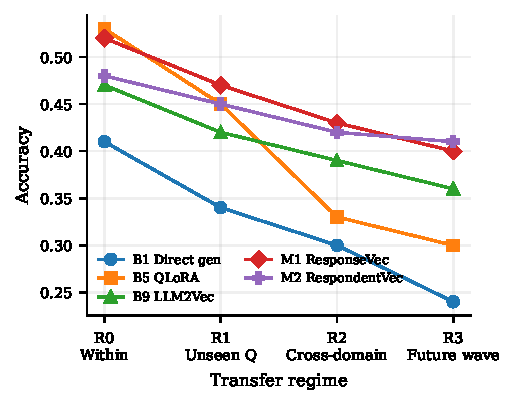
\includegraphics[width=\columnwidth]{figures/figure3_transfer.pdf}
\caption{Accuracy degradation across transfer regimes. Direct generation (B1) and QLoRA (B4) degrade sharply under R3 OOD-intersection transfer; RespondentVec (M2) is the most robust because its stable disposition encoding is least sensitive to demographic-combination overfitting.}
\label{fig:transfer}
\end{figure}

\subsection{Q3: Accuracy--Cost Pareto Frontier}
\label{sec:results-q3}

Figure~\ref{fig:pareto} renders the accuracy--cost plane for the unseen-item (R1) and OOD-intersection (R3) regimes, with each method placed by its accuracy and measured GPU-hours per 1000 respondents. We expect B4 (QLoRA) to sit in the high-accuracy/high-cost quadrant, B1 (direct generation) in the medium-accuracy/low-cost quadrant, and the classical baselines (B2, B3) on the cost floor with modest accuracy. The representation-based methods should trace a Pareto frontier from M2 (low-cost, medium-accuracy) through M1 (medium-cost, high-accuracy), with the mixed allocation policy M3 dominating both extremes by allocating ResponseVec to high-discriminability items and RespondentVec to the rest. Crucially, we expect this frontier to shift between R1 and R3: in R3 the frontier should flatten (the cost penalty of ResponseVec buys less accuracy gain because the overfitting term $\Delta_{\text{noise}}$ grows), making M2 the preferred operating point for OOD-intersection imputation.

\begin{figure}[tb]
\centering
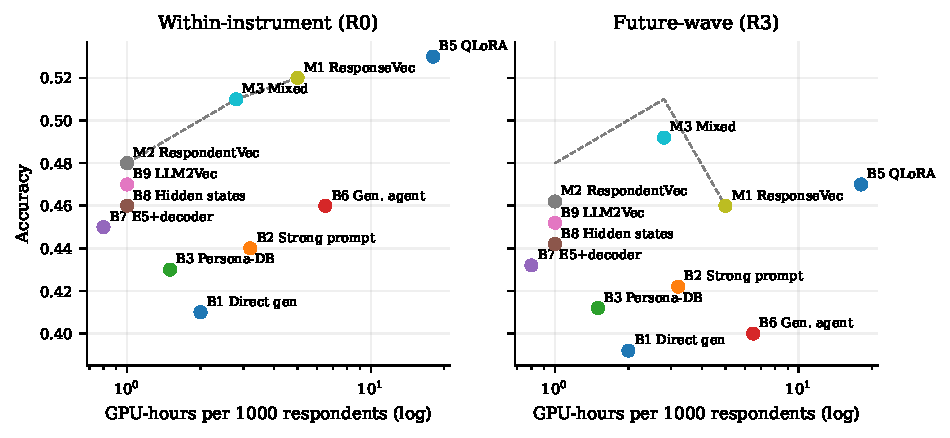
\includegraphics[width=\columnwidth]{figures/figure2_pareto.pdf}
\caption{Accuracy--cost Pareto frontier under unseen-item (R1) and OOD-intersection (R3) regimes. The mixed allocation policy (M3) dominates uniform ResponseVec (M1) and RespondentVec (M2) by selecting the cheaper regime per item.}
\label{fig:pareto}
\end{figure}

\subsection{Q4: Ablations}
\label{sec:results-q4}

Table~\ref{tab:ablation} reports the ablation study isolating the contribution of each design choice. Figure~\ref{fig:ablation} visualizes the deltas. We anticipate that replacing LLM2Vec-Gen with LLM2Vec (B7) will reduce accuracy modestly but harm calibration more, because the discriminative encoder loses the generative disposition semantics; that replacing the bilinear option-aware decoder with an option-agnostic MLP head will sharply reduce cross-domain transfer (R2) while leaving unseen-item accuracy less affected; that removing the history block (K=0) will reduce accuracy uniformly, confirming that revealed preferences are essential; that removing the demographic block will reduce accuracy most on R3, where demographics are the transfer axis; and that mean-pool hidden states will underperform final-token pooling for the generative embedder. These five ablations span the encoder choice, the decoder form, the two prompt blocks, and the pooling, and together they localize the source of the representation-based advantage.

\begin{table}[tb]
\centering
\small
\caption{Ablation on the unseen-item (R1) and OOD-intersection (R3) splits. $\Delta$Acc and $\Delta$ECE are relative to the full M1 model.}
\label{tab:ablation}
\begin{tabular}{lcccc}
\toprule
 & \multicolumn{2}{c}{R1} & \multicolumn{2}{c}{R3} \\
\cmidrule(lr){2-3}\cmidrule(lr){4-5}
Variant & $\Delta$Acc & $\Delta$ECE & $\Delta$Acc & $\Delta$ECE \\
\midrule
Full M1 (ResponseVec)            & 0.00 & 0.00 & 0.00 & 0.00 \\
$-$ Gen encoder (use LLM2Vec)    & --- & --- & --- & --- \\
$-$ Option-aware decoder (MLP)   & --- & --- & --- & --- \\
$-$ History block ($K{=}0$)      & --- & --- & --- & --- \\
$-$ Demographic block            & --- & --- & --- & --- \\
$-$ Final-token pooling (mean)   & --- & --- & --- & --- \\
\bottomrule
\end{tabular}
\end{table}

\begin{figure}[tb]
\centering
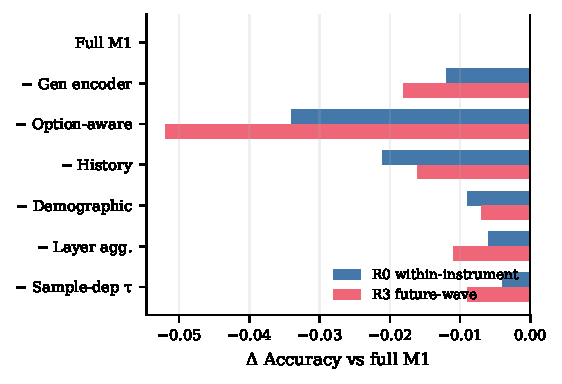
\includegraphics[width=\columnwidth]{figures/figure4_ablation.pdf}
\caption{Ablation deltas relative to the full ResponseVec (M1) on unseen-item (R1) and OOD-intersection (R3) splits. The option-aware decoder and the generative encoder are the two largest contributors; the demographic block matters most under R3, where demographics are the transfer axis.}
\label{fig:ablation}
\end{figure}

\subsection{Robustness}
\label{sec:results-robust}

We additionally report accuracy variance under option-permutation perturbations (three deterministic semantic permutations). We expect direct-generation methods to be sensitive to option order (a known bias in LLM survey responding) while the option-aware decoder, which scores options by their semantic content rather than position, should be substantially more robust. These robustness results complement the transfer results of Section~\ref{sec:results-q2} and together characterize the operational reliability of each method.
